\chapter{Marco Teórico - Tecnologías Web}
\label{chap2:MT}

\textbf{Nota:} En la sección \ref{Glosario} se encuentran conceptos básicos que el lector podría encontrar necesarios antes de empezar este trabajo.

\section{Arquitectura Cliente/Servidor}
    \label{chap2:ArqCS}
    La web emplea lo que se conoce como una Arquitectura Cliente-Servidor, donde la comunicación entre ambas entidades se basa mediante mensajes de \textit{request-response} o solicitud-respuesta. Con el tiempo la forma en que se comunican estos programas ha cambiado, desde iniciar solicitudes de forma secuencial e independiente, hasta solicitar asíncronamente varias peticiones. La evolución que ha tenido el cliente web ha permitido una mejor experiencia para el usuario, pero que conlleva ciertos riesgos que es necesario que el que usa el \textit{Browser} esté consciente. De la misma manera que podemos afectar a un servidor a través de las solicitudes, las respuestas que el servidor envía al cliente pueden tener consecuencias graves \cite{alcorn2014browser}.


\section{Comunicación e Información de Estado}

    \subsection{HTTP: Hypertext Transfer Protocol}
    \label{chap2:HTTP}
    El Protocolo de la capa de Aplicación conocido como HTTP fue creado en los años 90 por el \textbf{World Wide Web Consortium} \cite{w3c} y la \textbf{Internet Engineering Task Force}, define una sintaxis y semántica que utilizarían el software basado en una arquitectura Web para comunicarse. El protocolo sigue un esquema de solicitud-respuesta o \textit{request-response}, donde un cliente solicita un recurso que el servidor posee, y el servidor entrega una respuesta de acuerdo al recurso solicitado. La forma en que se localiza un recurso es mediante la dirección URL o \textit{Uniform Resource Locator}

        \subsubsection{Canales de comunicación en HTTP}
        \label{chap2:comunHTTP}
        Cuando se habla de HTTP usualmente ésto se relaciona con la comunicación que se lleva a cabo entre el cliente y servidor. Existen diversas formas para que esto se lleve a cabo, las más conocidas son:
        \begin{enumerate}
            \item postMessage \cite{webMessaging}: Mecanismo de comunicación entre ventanas y frames, disponible en la API de HTML5, entre diversos dominios. El comando window.postMessage es usado para realizar llamadas entre diversos orígenes de forma segura. Si bien SOP normalmente denega este tipo de solicitud, si se hace de forma correcta es posible cominicarse con diversos orígenes por medio del uso de este comando.

            \item XMLHttpRequest o XHR: \cite{XHR} define una API que proporciona una guía de funcionalidad al cliente, para que éste pueda transferir datos del cliente al servidor. Dicho de otra manera, XHR es un objeto que permite la obtención de recursos en la Internet. Soporta peticiones en HTTP o HTTPS, en general soporta toda actividad relacionada con un \textit{HTTP request or response}, para los métodos definidos.

            \item WebSockets \cite{WebSocket}: Es una tecnología nativa del navegador que permite abrir un canal de comunicación interactivo, responsivo y \textit{full-duplex} entre el cliente y el servidor. Éste comportamiento permite tener \textit{event-driven actions} rigurosas sin necesidad explícita de sondear el servidor en todo momento. Websockets intenta reemplazar las tecnologías \textit{Push} basada en AJAX.

            \item WebRTC \cite{WebRTC}: O mejor conocido como \textit{Web Real-Time Communication}, es una API basada en la especificcación de la W3C, que utiliza las capacidades de Javascript y HTML5 (sin la utilización de plugins externos o internos) para transmitir audio, video y compartir archivos por medio de P2P. Esta herramienta permite a los browsers comunicarse entre ellos a muy baja latencia y entrega un gran ancho de banda/\textit{bandwidth} para poder realizar comunicaciones multimedia en tiempo real. Hasta el momento Google Chrome/Chromium y Firefox han implementado esta tecnología, con el objetivo de: mejorar la experiencia de usuario al no necesitar plugins para ser usada, y entregar seguridad dado que impone el uso de cifrado en los datos.
        \end{enumerate}

    \subsection{SSL/TLS Cifrado en capa de Transporte}
    Si bien existe una medida de seguridad en los headers que se implementa en la capa de Aplicación por medio de HTTP, esto no impide que otros puedan ver qué contienen los paquetes. La confidencialidad, autenticidad y el no repudio de lo que se envía, es un aspecto relevante cuando se está trabajando con sistemas con información crítica y confidencial. SSL (Secure Socket Layer) y TLS (Transport Layer Security) \cite{RFC-5246} tienen el objetivo de proveer un canal confiable y privado de todo lo que se envía entre dos aplicaciones que se comunican; es una seguridad \textit{end-to-end}. TLS es el resultado de la estandarización de SSL por la Internet Engineering Task Force (IETF). SSL/TLS trabaja debajo del protocolo HTTP, usando certificados de clave pública que permiten:
    \begin{itemize}
        \item Resolver parcialmente el problema de la autenticación de un usuario, al establecer un canal seguro y cifrado mediante el uso de certificados digitales.
        \item Identificar que la información enviada por los dos \textit{endpoints} sea solo de ellos dos, agregando una firma al final del paquete usando la clave privada de la entidad que envía.
        \item Asegurar que todo lo que se envía sea visto sólo por las entidades que crean el canal de comunicación, a través del cifrado y descifrado.
    \end{itemize}

    El proceso que permite el inicio de una comunicación mediante SSL/TLS es:
    \begin{enumerate}
        \item Un usuario desea conectarse por el \textit{Browser} a un Web Server.
        \item Se inicia el proceso de \textit{Handshake} entre el \textit{Browser} y Servidor. Éstos dos se ponen de acuerdo en cómo se cifrará la comunicación (parámetros e información de los certificados) e intercambian una llave asimétrica.
        \item El navegador valida el certificado, ejemplo: revisa si está expirado, revocado o fue creado por una CA \textit{Certificate Authority} confiable.
        \item Si el servidor requiere un certificado por parte del cliente, el \textit{Browser} le enviará el suyo. Esto permitirá tener una autenticación mutua entre las partes.
        \item El \textit{Web Browser} y el Servidor usan las llaves públicas del otro para poder acordar una clave simétrica, que es aquella que permitirá cifrar los mensajes. Sólo estas dos entidades conocerán tal clave.
        \item El proceso de \textit{handshake} termina y todo lo posterior se realiza cifrando los paquetes con la llave simétrica acordada por las partes.
    \end{enumerate}

    Para que tanto SSL y TLS provean una conección segura, todos los componentes involucrados (cliente, servidor llaves y aplicación web) deben ser seguros.

    \subsection{Speedy o Protocolo SPDY}
    \label{chap2:spdy}
    Es un protocolo de red abierto desarrollado por Google en el 2009, para el transporte de contenido Web. A modo general utiliza técnicas de \textit{multiplexing}, compresión y priorización. Sin embargo, depende bastante de las condiciones del sitio web y su despliegue en la red. SPDY manipula el tráfico en el protocolo HTTP para disminuir el tiempo de carga de las páginas web, al mismo tiempo que cuida la seguridad de los datos. Este protocolo modifica la forma en que las peticiones y respuestas HTTP son enviadas a la Internet (por el cable); SPDY es considerado una especie de tunel. Sin embargo, cuando la versión 2 de HTTP esté completa SPDY quedará obsoleta. Implementaciones de este protocolo se dan en: Google Chrome/Chromium, Internet Explorer, Firefox, Safari, Opera y Amazon Silk.
    

    %Ver libro de Browser hacker handbook
\section{Tecnologías usadas}

    \subsection{Markup Languages}
    \label{chap2:markup}
        Un lenguaje de marcado sigue tradicionalmente un \textit{Standard Generalized Markup Language}, de manera que entrega una semántica apropiada para representar o mostrar contenido, placeholders de aplicaciones y datos. Cada página mostrada por el navegador, sigue las instrucciones que el lenguaje de marcado le da al browser para mostrar el contenido. HTML y XML son los más conocidos en el mercado. Ambos lenguajes tienen sus especificaciones en la W3C o \textit{World Wide Web Consortium}.

        \subsubsection{HTML: HyperText Markup Language}
        \label{chap2:HTML}
        HTML \cite{htmlSpec}, en especial la actual versión HTML5, es conocido por ser un \textit{Simple Markup Language} o lenguage de marcado simple, usado principalmente para crear documentos de hypertextos que son posibles de portar desde una plataforma a otra, sin problemas de compatibilidad. Un documento HTML consiste de un árbol de elementos y texto, cada uno de esos elementos es denotado por un \textit{tag}/etiqueta inicial y uno final; estos \textit{tags} pueden ir anidados y la idea es que no se superponen entre ellos. Un HTML User Agent o \textit{Browser} consume el HTML y lo parsea para crear un árbol DOM, que es la representación en memoria del documento HTML.
        Una característica importante de este lenguaje de marcado es su flexibilidad ante los errores, esto es que en alguna ocasiones el programador perfectamente podría sobrarle un signo y HTML no le daría mayor importancia mientras no afecte a la estructura global de la página. Normalmente esta característica es aprovechada por los atacantes para insertar nuevos elementos HTML que ejecuten scripts que afectarían al navegador.


        \subsubsection{XML: eXtensible Markup Language}
        \label{chap2:XML}
        Este lenguaje de marcado tiene una estrecha relación con HTML, pero a diferencia de este último tiene una sintáxis y semántica más rígida ya que sigue al pie de la letra un lenguaje libre de contexto. Este tipo de lenguaje es ideal para el transporte de datos entre \textit{web Services} o interacciones \textbf{RPC}, dado que no hay forma de como malinterpretar los datos.


    \subsection{CSS: Cascading Style Sheets}
    \label{chap2:css}
    Es un lenguaje usado junto a HTML o XML para definir la capa de presentación de las páginas web que el navegar renderiza al usuario. La W3C se encarga de la especificación de las hojas de estilos para que los browser sean capaces de interpretar bajo estándares y aseguren ciertos niveles de calidad. Una hoja de estilo se compone de una lista de reglas. Cada regla o conjunto de reglas consiste en uno o más selectores y un bloque de declaración, más los estilos a aplicar para los elementos del documento que cumplan con el selector que les precede. 


    \subsection{DOM: Document Object Model}
    \label{chap2:DOM}
    Es una \textit{API} independiente del lenguage y multiplataforma para HTML válido y bien formado, que define la estructura lógica de un documento que permite ser accedido y manipulado. DOM es una especificación que permite a programas Javascript modificar la estructura del contenido de una página dinamicamente. Esto permite que una página pueda cambiar sin la necesidad de realizar nuevas peticiones al servidor y sin la interacción del usuario. Posteriormente la \textit{W3C} \cite{w3c} formó el \textit{DOM Working Group} y con ello se creó la especificación a través de la colaboración de muchas empresas y expertos. La arquitectura de esta \textit{API} se presenta en la Figura \ref{fig:DOM}, donde el \textit{Core Module} es donde están las interfaces que deben ser implementadas por todas las implementaciones conformes de DOM. Una implementación de DOM puede ser construida por uno o más módulos dependiendo del host, ejemplo de esto: la implementación de DOM en un servidor, donde no es necesaria la implementación de los módulos que manejen los triggers de eventos del mouse.
            
    \begin{figure}[h!t]
            \centering
        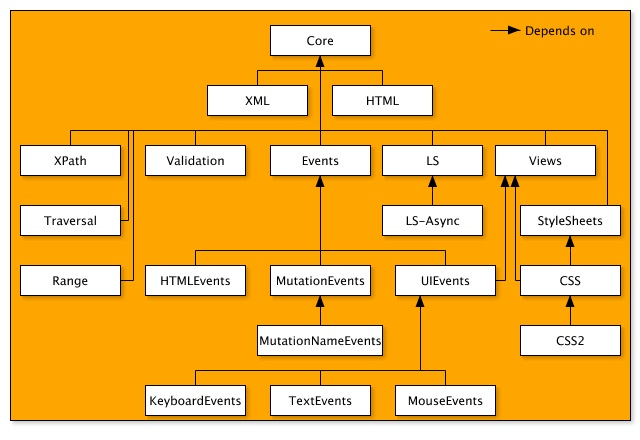
\includegraphics[width=0.7\textwidth]{figures/dom-architecture.jpg}
        \caption{Arquitectura de DOM. Fuente: \cite{w3c}}
        \label{fig:DOM}
    \end{figure}
            
    La interfaz de \textit{DOM} fue definida por el \textbf{OMG IDL} y fue construida para ser usada en una gran variedad de ambientes y aplicaciones. El documento parseado por DOM se transforma en un gran objeto, tal modelo captura la estructura del documento y el comportamiento de éste, además de otros objetos de lo que puede estar compuesto y las relaciones entre ellos. Cada uno de los nodos representa un elemento parseado del documento, el cual posee una cierta funcionalidad e identidad. La estructura de árbol del DOM construido puede llegar a ser gigantezca, y almacena más de un árbol por cada documento que parsea. 
            
    \subsection{Javascript, VBScript y otros}
    \label{chap2:JS}
    Ambos son lenguajes de scripting orientados a objetos. Javascript fue desarrollado por Netscape mientras que VBScript fue desarrollado por Microsft para Internet Explorer, los dos siguen el estándar del lenguage de scripting \textbf{ECMAScript}. Dado que VBScript no era usado por muchos y no tenía soporte para otros navegadores más que Internet Explorer, Microsoft decidió abandonarlo.

    Muchos piensan que JavaScript es un lenguage interpretado, pero es más que eso. Javascript es un lenguage de \textbf{scripting dinámico} (por tanto no tipificado) que soporta la construcción de objetos basados en \textbf{prototipos}. Esto quiere decir que a diferencia de un lenguage de programación orientado a objetos como Java, un lenguage orientado a prototipos no hace la distinción entre clases y objetos (clase instanciada), son simplemente objetos. Y cómo tal al ser construido con sus propidades iniciales, es posible poder agregar o remover propiedades y métodos de forma dinámica (durante el runtime) tanto a un objeto como a la clase.
            
    Javascript puede funcionar tanto como un lenguage de programación procedural o como uno orientado a objetos. Firefox usa una implementación en C de Javascript llamada \textit{Spider Monkey}, Google Chrome/Chromium tiene un motor de JavaScript llamado \textit{V8}, e Internet Explorer no usa realmente JavaScript, sino que \textit{JScript} (hace lo mismo que las otras implementaciones solo que difiere en el sistema operativo que utiliza) que en este caso se llama \textit{Chakra}.
            
    Si bien es posible comprender que JavaScript posee increíbles posibilidades para la creación de \textit{RIA} (Rich Internet Applications), en \cite{barth2009attacks, Barth2009, Barth2010, Liu2012, Singh2014} se muestran que puede llegar a ser un fracaso si es que no se toman en cuenta ciertas vulnerabilidades inherentes al lenguage. Estas vulnerabilidades que pueden llegar a ser críticas, a menudo permiten a un comunicante comprometer completamente a la otra parte. La misma naturaleza de JavaScript que permite la modificación en runtime de los objetos, puede llegar a ser aprovechada de esta situación; en la cita toma por ejemplo la comunicación entre los elementos de un \textit{Mashup}.


    \subsection{Geolocalización}
    Cada \textit{Browser} posee una API que permite obtener los datos de la localización del host donde el browser está alojado. Ésta es obtenida ya sea del GPS, si es un dispositivo móvil, como de la triangulación de la señal del celular, localización de IP del movil o \textit{access point}.

    \subsection{WebWorkers}
    \label{chap2:WWs}
    Ésta tecnología permite la creación de \textit{threads} en el browser para separar las tareas de éste, dejando algunas en el \textit{background} para incrementar el rendimiento total de la carga de las páginas web. La API permite que el autor de una aplicación web, ejecute \textit{trabajadores} que corren scripts en paralelo, la coordinación entre éstos se logra a través del paso de mensajes. Existen 2 tipos: una que es compartida por todo aquello de un mismo \textbf{Origen} y otra que se comunica hacia atrás a la función que la creó. Esta API entrega al desarrollador más flexibilidad, pero que sin duda los atacantes también aprovechan bastante.


\section{Desafíos del Navegador}
    \label{chap2:Desafios}
    \begin{itemize}
        \item Navegación a todo tipo de contenidos/compatibilidad: sin importar el esquema de la página web, el navegador debe ser capaz de presentar todo tipo de contenido al usuario. \cite{barth2008security} asegura que los usuarios demandan compatibilidad, por que el browser es sólo útil mientras pueda mostrar las páginas.
        \item Navegación personalizada: el browser debe ser capaz de entregar la información a la Web Aplicación/sistema, para que identifique al usuario por detrás, de manera que la navegación sea personalizada.
        \item Navegación sin inconvenientes: el navegador debe ser capaz de aislar los errores que se presenten en algunas páginas, de tal manera que no molesten a las otras páginas web que se ven al mismo tiempo \cite{IE8-LCIE, preprint-grosskurth-browser-archevol, barth2008security}
        \item Seguridad: Los datos de los usuarios y el host donde se mantiene el \textit{Browser} no deben ser expuestos a terceras partes \cite{Reis2009, barth2009securing, Barth2010, Liu2012, barth2009attacks, Saini2014}.
    \end{itemize}


%%%%%%%%%%%%%%%%%%%%%%%%%%%%%%%%%%%%


\section{Arquitectura de Referencia o Reference Architecture (AR)}
\label{chap2:ArqRef}
%usar \cite{Avgeriou2003}

Una arquitectura de Referencia, de acuerdo a la \textit{Open Security Architecture} o OSA \cite{openSecArch}, es considerado un elemento que describe un \textbf{estado de ser} y debe representar aceptadas buenas prácticas. En \cite{Avgeriou2003, Galster2011a} se explica que una AR es una arquitectura de software genérica y estandarizada, para un dominio particular e independiente de la plataforma o detalles de implementación. En ésta especifica la decomposición del sistema en subsistemas, las interacciones entre estas partes y la distribución de funcionalidad entre ellas \cite{Bass2012}. 

Actualmente no hay un consenso de cómo definir una AR, lo que debería contener y cómo debería de construirse \cite{Avgeriou2003, Galster2011a} describe un ejemplo e indica cómo debería de ser ésta, con los siguientes elementos:
\begin{itemize}
    \item Describir los Stakeholders que interactuan con el sistema y que poseen preocupaciones/\textit{concerns} de éste.
    \item Generar \textit{views} usando UML y teniendo en cuenta un proceso \textit{Rational Unified Process}: crear casos de uso, modelos de análisis y diseño, modelo de despliegue e implementación.
    \item Patrones de Arquitectura.
    \item Atributos de calidad deseables que el sistema debe garantizar. Es importante solo destacar aquellos realmente necesarios, dado que un sistema sobrecargado con ellos tampoco es conveniente.
\end{itemize}

Las ventajas y usos que se obtienen al construir una AR en este trabajo son:
\begin{itemize}
    \item Comprender la estructura subyacente de un \textit{Web Browser} y las interacciones que tendrá con otros sistemas.
    \item Proveer una base tecnológica modular y flexible. Al tener los subsistemas compartimentalizados es posible quitar y sacar piezas, que poseen interfaces similares, y de esa manera reusar lo otro sin tener que construir un sistema nuevo.
    \item Entrega una base para el desarrollo de otros Navegadores Web, sin explicar detalles de implementación.
\end{itemize}

En este trabajo el enfoque estará en el primer punto, donde se quiere entender las interacciones entre un desarrollo de Software y la utilización de las funcionalidades del navegador. Dado que parte de la investigación es obtener Patrones de Mal Uso o Uso Indebido del navegador Web, es primordial concebir una Arquitectura de Referencia que permita encontrar dónde es posible aplicar Patrones de seguridad para poder mitigar los malos usos del \textit{Browser} \cite{Submitted2014}. 

Una AR es una herramienta que facilita el entendimiento de sistemas complejos y la apropiada implementación a sistemas reales. Si bien una AR es usada principalmente para capturar las preocupaciones de los \textit{Stakeholders} al comienzo de un Desarrollo de Software, también puede ser usada para educar al realizar la unión de ideas y terminologías usadas por diversos sistemas que se asemejen. Una Arquitectura de Referencia debe ser en lo posible descrita de la forma más abstracta posible, pues su función de guiar la construcción de arquitecturas concretas, sin tener en cuenta detalles de las tecnologías usadas. 

\subsection{Validación de la Arquitectura}
    \cite{Galster2011a} menciona que existe una falta de procedimientos para diseñar sistemáticamente una Arquitectura de Referencia, que sea al mismo tiempo fundamentada empíricamente. El mismo trabajo explica que mientras un Arquitecto de Sistema y un Experto de Dominio trabajen juntos, es posible diseñar AR ya sea desde \textit{cero} o basado en artefactos arquitecturales ya existentes. Para una AR no construida desde el comienzo, la evaluación es menos crítica dado que la AR utiliza conceptos arquitecturales ya comprobados por expertos. Por lo tanto, la validación de ésta puede derivarse desde arquitecturas ya construidas, en este caso a partir de los browser que se encuentran en el mercado.

    Para describir la Arquitectura de Referencia nos hemos basado en los trabajos \cite{Hashizume2014Reference, Submitted2014}, usando patrones para la contrucción de la AR. Así como indica \cite{Bass2012}, es posible usar patrones arquitecturales para diseñar una Arquitectura de Referencia, con tal de obtener atributos de calidad deseados.



\section{Desarrollo de Software Seguro y Diseño de Software Seguro}
\label{chap2:SSD}

La filosofía detrás de \textit{Secure Software Development} es que detrás de cada etapa de desarrollo del software, se tengan en cuenta los prinicipios de seguridad: confidencialidad, integridad, disponibilidad y auditoría. Para cumplir este cometido es que se deben llegar a políticas y reglas que aseguren la seguridad como una propiedad sistémica.

Varias comunidades tienen diferentes enfoques y técnicas de cómo asegurar la seguridad en los sistemas, muchas pueden incluso tener similitudes y hasta trabajar juntas. En este trabajo, el enfoque tomado es aquel que busca entregar la propiedad de seguridad a través del entendimiento de un sistema a un alto nivel, identificando las amenazas durante la elicitación de requerimientos, de manera que se pueda extraer las posibles amenazas que podrían existir y utilizando elementos de diseño para hacer cumplir los principios de seguridad necesarios por el sistema; este enfoque es el que se dedica la comunidad de \textit{Secure Software Design}. 

Fernandez \cite{Fernandez2011a,fernandez2013security} sostiene que para construir un sistema seguro es necesario realizarlo de manera sistemática de tal manera que la seguridad sea parte integral de cada una de las etapas del Desarrollo de Software - de inicio a fin. El enfoque que propone es ingenieril y, por tanto, es aplicable incluso para sistemas \textit{legacy}, donde es posible hacer ingeniería inversa para comprobar si existen o no los requerimiento de seguridad implementados, de manera que permite generar un estudio con la intención de comparar y mejorar nuevos sistemas. Fernandez en su libro \cite{fernandez2013security} presenta una completa metodología para construir sistemas seguros a partir del Diseño Orientado a Objetos, UML y patrones, a los cuales nombra como \textbf{Security Patterns}.

Como parte de la metodología propuesta, se plantea que para diseñar primero se deben entender las posibles amenazas a las que está expuesto el sistema. La identificación de Amenazas \cite{braz2008eliciting,fernandez2006defining} es la primera tarea que presenta la metodología, que considera las actividades en cada caso de uso del sistema.


\section{Patrones}
\label{chap2:Patt}
Los Patrones encapsulan soluciones recurrentes a problemas y definen una forma de expresar los requerimientos y soluciones de una forma concisa, al mismo tiempo que proveen de un vocabulario común entre los diseñadores \cite{buschman1996system}. Un patrón encarna el conocimiento y experiencia de desarrolladores de software que puede ser reusado posteriormente en nuevas aplicaciones \cite{fernandez2004methodology, Fernandez2006, Fernandez2011, fernandez2013security}. Los Patrones expresan las relaciones entre un contexto, un problema y una solución. Para un contexto dado, el patrón puede ser adaptado para encajar en diversas situaciones. La construcción de Patrones de Seguridad parte de la premisa anterior, éste permite construir sistemas seguros a través del uso de Patrones adaptados a las necesidades del sistema y preocupaciones de los \textit{Stakeholders}. Por otra parte, una Arquitectura puede ser descrita a través de Patrones, permitiendo que haya un mejor entendimiento al momento de proveer con guías de diseño y análisis a desarrolladores.

Los patrones describen diseños recurrentes en un mediano nivel de abstracción y es poco probable que existan solos; existen en conjunto a otros patrones. Un patrón puede proveer una solución usando diagramas en UML, de manera que describen de forma precisa al sistema.

La Arquitectura de Referencia a confeccionar será realizada por medio de patrones y éstos serán descritos con el template creado por \cite{buschman1996system}, llamado POSA, que contiene las siguientes secciones para describir un patrón: \textit{Intent}, Contexto, Problema, Solución, Implementación, Usos comúnes, Consecuencias y Patrones relacionados.




%\section{Patrones de Seguridad}
%\label{chap2:SecPatt}
%Los Patrones de Seguridad son aquellos que encarnan buenos principios de diseño que tienen en cuenta ciertos principios de seguridad, y que al ser aplicados en una metodología para el desarrollo de sistemas, es posible asegurar que el sistema aplique esos principios y en consecuencia generar un sistema seguro \cite{fernandez2004methodology, fernandez2013security}. Estos patrones describen las maneras de detener o mitigar una posible amenaza de seguridad, especificando una solución a través de mecanismos de seguridad, para el contexto dado. Las soluciones propuestas deben resolver las fuerzas o \textit{forces} indicadas por el patrón. Un uso importante de estos patrones es la ayuda que aportan a desarrolladores que no son expertos en seguridad; éstos permiten ayudarlos a implementar mecanismos que implementen los principios de seguridad necesarios.

\section{Patrones de Mal Uso}
Para diseñar sistemas seguros, se es necesario identificar las posibles amenazas que un sistema puede sufrir. Papers como \cite{fernandez2006defining, fernandez2007attack, braz2008eliciting, fernandez2013security} describen el desarrollo de una metodología completa para encontrar amenazas, a través del análisis de actividades de los casos de uso del sistema, buscando como podría un atacante interno o externo socavar las bases de esas actividades. Es importante no confundir \textit{Attack Patterns} con \textit{Misuse Pattern}, pues claramente en \cite{ModMisusePatt, fernandez2013security} dejan explícito que un \textit{Attack Patttern} es una acción que lleva a un mal uso o \textit{misuse}, o acciones \textbf{específicas} que toman ventaja de las vulnerabilidades de un sistema, como por ejemplo un \textit{buffer overflow}. A partir de los trabajos \cite{fernandez2007attack, yoshioka2006development, yoshioka2007integration}  se hace la unión de los conceptos de \textit{Attack Patttern} para dar forma a la definición de \textit{Misuse Pattern} \cite{ModMisusePatt, pelaez2009misuse, fernandez2010worm, hashizume2011misuse, munoz2011misuse, fernandez2012misuse, alkazimi2014, encinamisuse}:
\begin{center}
    Un patrón de mal uso o \textit{Misuse Pattern} describe desde el punto de vista del atacante, cómo un tipo de ataque es realizado (qué unidades usa y cómo), analiza las maneras de detener el ataque através de la enumeración de posibles Patrones de seguridad que pueden ser aplicados, y describe cómo rastrear un ataque una vez que ha ocurrido por medio de una recolección y observación apropiada de datos forenses.
\end{center}

Sin embargo, cuando un sistema ya está diseño y construido, como es el caso del \textit{Web Browser}, lo que va a importar es saber \textbf{cómo} los componentes del sistema, pueden ser usados por el atacante para alcanzar sus objetivos. Importante es entender que éste patrón describe un contexto en dónde puede ocurrir el ataque.

Un catálogo de \textit{Misuse Patterns} podría ser de gran valor en el Desarrollo de Sistemas que interactúan con el navegador, pues provee a desarrolladores un medio para evaluar los diseños de sus sistemas, al analizar las posibles amenazas del \textit{Browser} que pudieran afectar al software que está siendo construido.
